%%%%%%%%%%%%%%%%%%%%%%%%%%%%%%%%%%%%%%%%%%%%%%%%%%%%%%
% This code is a template for a presentation
% feel free to edit it and use it
% Author  : D. Chibouti
% Contact : dchibouti@gmail.com
% github  : https://github.com/dchibouti
% date    : 20 June 2022
%%%%%%%%%%%%%%%%%%%%%%%%%%%%%%%%%%%%%%%%%%%%%%%%%%%%%%

%\documentclass[10pt,t]{beamer}
\documentclass[aspect ratio=169,t]{beamer}
%%%%%%%%%%%%%%%%%%%%%%%%%%%%%%%%%%%%%%%%%%%%%%%%%%%%%
%%% Version imprimable sous forme document 
%------------------------------------
% \documentclass[10pt]{article}
% \usepackage{beamerarticle}
% \usepackage[a4paper]{geometry}
% \geometry{verbose,tmargin=3cm,bmargin=3cm,hmargin={3cm,3cm}} 
%%%%%%%%%%%%%%%%%%%%%%%%%%%%%%%%%%%%%%%%%%%%%%%%%%%%%

\usepackage{lmodern}        %Polices vectorielles %!!!

%------------------------------------
\usepackage{hyperref}
\hypersetup{
	colorlinks=false,       % false: boxed links; true: colored links
	linkcolor=blue,          % color of internal links (change box color with linkbordercolor)
	citecolor=blue        % color of external links
}
%------------------------------------

\usepackage{graphicx}
%\usepackage{movie15}
\usepackage[playbutton=fancy]{media9}

\usepackage{animate}

%\usetheme{Warsaw}
%\useoutertheme{shadow}
%\setbeamertemplate{headline}{}
%\setbeamertemplate{navigation symbols}{}
%\setbeamercolor{frametitle}{bg=black,fg=structure.fg}
\usetheme{Madrid}
%\usecolortheme{beaver}


\newcommand{\couleur}{blue!65!black}
%\definecolor{amber}{rgb}{1.0, 0.49, 0.0}
\definecolor{amber}{rgb}{0.04706, 0.03725, 0.26667}
%\definecolor{amber}{rgb}{0.04706, 0.03725, 0.4526667}


\renewcommand{\couleur}{amber!98!black}
%\newcommand{\couleur}{amber}
\setbeamercolor{structure}{fg=\couleur!100,bg=\couleur!0}
\colorlet{macouleur}{\couleur}

\usepackage{multimedia}


%\useinnertheme{rectangles}
%\useoutertheme{infolines}


\setbeamertemplate{footline}[frame number]
\setbeamersize{text margin left = 0.5cm, text margin right = 0.5cm}

\setbeamertemplate{navigation symbols}{}

\renewcommand{\figurename}{{Fig.}}
\usepackage[labelsep=endash]{caption}
\setbeamertemplate{caption}[numbered]
\renewcommand{\vec}[1]{\mathbf{#1}}


%------------------------------------
%%%  COMMANDES COULEURS
%------------------------------------
\newcommand\montre[1]{\textbf{\color{\couleur}{#1}}}
\newcommand\colorise[1]{{\color{\couleur}{#1}}}
%------------------------------------
%%%%%%%%%%%%%%%%%%%%%%%%%%%%%%%%%%%%%%%%%%%%%%%%%%%%%%
\newcommand\blue[1]{\textcolor{blue}{#1}} %!!!
\newcommand\red[1]{\textcolor{red}{#1}} %!!!
\newcommand\green[1]{\textcolor{green}{#1}} %!!!
\newcommand\orange[1]{\textcolor{orange}{#1}} %!!!
\newcommand\magenta[1]{\textcolor{magenta}{#1}} %!!!
\renewcommand{\thefootnote}{\roman{footnote}}
\renewcommand{\vec}[1]{\mathbf{#1}} % vecteurs %!!!

%%%%%%%%%%%%%%%%%%%%%%%%%%%%%%%%%%%%%%%%%%%%%%%%%%%%
\usepackage{stmaryrd}
\newcommand{\rp}{\right)} % right parenthesis
\newcommand{\lp}{\left(} % left parenthesis

\newcommand{\rd}{\right} % right
\newcommand{\ld}{\left} % right parenthesis

%%%%%%%%%%%%%%%%%%%%%%%%%%%%%%%%%%%%%%%%%%%%%%%%%%%%%%
%                Boxes                               %
%%%%%%%%%%%%%%%%%%%%%%%%%%%%%%%%%%%%%%%%%%%%%%%%%%%%%%
\usepackage{xcolor}
\newcommand{\mybox}[1]{\fbox{$\displaystyle#1$}}
\newcommand{\myredbox}[1]{\fcolorbox{red}{white}{$\displaystyle#1$}}
\newcommand{\mybluebox}[1]{\fcolorbox{blue}{white}{$\displaystyle#1$}}
\newcommand{\mygreenbox}[1]{\fcolorbox{green}{white}{$\displaystyle#1$}}
\newcommand{\myvioletbox}[1]{\fcolorbox{violet}{white}{$\displaystyle#1$}}
\newcommand{\myblackbox}[1]{\fcolorbox{black}{white}{$\displaystyle#1$}}
\newcommand{\mydoublebox}[1]{\fbox{\fbox{$\displaystyle#1$}}}
\newcommand{\myreddoublebox}[1]{\fcolorbox{red}{white}{\fcolorbox{red}{white}{$\displaystyle#1$}}}

%%%%%%%%%%%%%%%%%%%%%%%%%%%%%%%%%%%%%%%%%%%%%%%%%%%%


%------------------------------------
\usepackage{tikz}
\usetikzlibrary{calc}
\usetikzlibrary{arrows}
% tikz perspective
\tikzset{math3d/.style={x={(-0.353cm,-0.353cm)},z={(0cm,1cm)},y={(1cm,0cm)}}}
\usetikzlibrary{3d}
\usetikzlibrary{decorations.pathreplacing}
\usepackage{pgfplots}
\usepackage{subfigure}
%------------------------------------

%------------------------------------
% maths
%------------------------------------
\usepackage{amsthm,amsfonts,amssymb}
\usepackage{mathrsfs}
\usepackage{amsmath}
%\usepackage[fleqn]{amsmath}
%\setlength\mathindent{0pt}
%------------------------------------
\numberwithin{equation}{section} % numero equations
\usefonttheme[onlymath]{serif}
%------------------------------------

\newtheorem{lemm}{Lemme} % La petite étoile enlève la numérotation, maisnécessite le package amsthm
\newtheorem{prop}{Proposition}    
\newtheorem{defi}{Définition}
\newtheorem{theo}{Théorème}
\newtheorem{rema}{Remarque}
\newtheorem{rapp}{Rappel}
\newtheorem{enon}{\'Enoncé}
\newtheorem{bloc}{}



%------------------------------------
%%%%%%  suite listes
%------------------------------------
\newcounter{sauvegardeenumi}
\newcommand{\asuivre}{\setcounter{sauvegardeenumi}{\theenumi}}
\newcommand{\suite}{\setcounter{enumi}{\thesauvegardeenumi}}
%------------------------------------


%------------------------------------
% changement numerotation titre si allowframebreak
%------------------------------------
%%\setbeamertemplate{frametitle continuation}{[\insertcontinuationcount]}
%\setbeamertemplate{frametitle continuation}{}
\setbeamerfont{title}{series=\bfseries,parent=structure}
\setbeamerfont{frametitle}{series=\bfseries,parent=structure}
%%%%%%%%%%%%%%%%%%%%%%%%%%%%%%%%%%%%%%%%%%%%%%%%%%%%%

\usepackage{listings}

\lstset{
	language=Fortran,
	basicstyle=\ttfamily\small,
	breaklines=true,
	prebreak=\raisebox{0ex}[0ex][0ex]{\ensuremath{\hookleftarrow}},
	frame=lines,
	showtabs=false,
	showspaces=false,
	showstringspaces=false,
	keywordstyle=\color{blue},%\bfseries,
	stringstyle=\color{magenta},%!50!black
	commentstyle=\color{gray}\itshape,
	%	numbers=left,
	captionpos=b,
	escapeinside={\%*}{*)}
}

\usepackage{cancel}

% Table des matières qui apparaît au début de chaque division :
\AtBeginSection{%
	\begin{frame}
		\frametitle{Table of contents}
		\tableofcontents[sectionstyle=show/shaded,subsectionstyle=hide,subsubsectionstyle=hide]
	\end{frame}
}
%%%%%%%%%%%%%%%%%%%%%%%%%%%%%%%%%%%%%%%%%%%%%%%%%%%%%

%%%%%%%%%%%%%%%%%%%%%%%%%%%%%%%%%%%%%%%%%%%%%%%%%%%%%

\title{\textbf{Notes/Results}}
%\author{\textbf{D. Chibouti}}



%%%%%%%%%%%%%%%%%%%%%%%%%%%%%%%%%%%%%%%%%%%%%%%%%%%%%
%   Title page customized
%%%%%%%%%%%%%%%%%%%%%%%%%%%%%%%%%%%%%%%%%%%%%%%%%%%%%
\setbeamerfont{Hl text}{series=\bfseries}


{
  \usebeamerfont{subtitle}\usebeamercolor[fg]{subtitle}\insertsubtitle\par
  \bigskip
  \usebeamerfont{author}\insertauthor\par
  \usebeamerfont{institute}\insertinstitute\par
  \usebeamercolor[fg]{titlegraphic}\inserttitlegraphic
}
\title{\huge{Result notes} }
\subtitle{coupling strategy}
\author{\textcolor{black}{\text{D. Chibouti}, B. Trouette, C. Chénier}}
\institute{Univ Gustave Eiffel, Univ Paris Est Créteil, CNRS, UMR 8208, MSME, \\ F-77454 Marne-la-Vallee, France}
\date{\textcolor{blue}\today}




\begin{document}
%%%%%%%%%%%%%%%%%%%%%%%%%%%%%%%%%%%%%%%%%%%%%%%%%%%%%
%   first page (Title page)
%%%%%%%%%%%%%%%%%%%%%%%%%%%%%%%%%%%%%%%%%%%%%%%%%%%%%

{
% \usebackgroundtemplate{
\includegraphics[width=\paperwidth]{figures/bg.png}}
\usebackgroundtemplate{
\includegraphics[width=\paperwidth]{figures/background.jpg}}
\begin{frame}[noframenumbering, plain]
\maketitle
\end{frame}
}

%%%%%%%%%%%%%%%%%%%%%%%%%%%%%%%%%%%%%%%%%%%%%%%%%%%%%
%   Columns
%%%%%%%%%%%%%%%%%%%%%%%%%%%%%%%%%%%%%%%%%%%%%%%%%%%%%
\begin{frame}{Rappels -- Basis and analytical functions}
\begin{equation*}
    \frac{{\rm d}  u(z)}{{\rm d} z}= {\frac { {\it {\blue{u}}-u_p} }{ h_{K}+{\sigma_u\,\red{\lambda}}} } \quad ; \quad {\red{\lambda}} = {\frac {\mu}{\red p}} \sqrt {\frac {\pi}{2} r {\it T}}
    \label{eq:pente_analytique}
\end{equation*} 
%%%%
\begin{equation*}
\phi^{(1)}{({x})}~=~\ld\{ x^{-i}\vert i\in \llbracket0,M_1\rrbracket\rd\}
\quad ; \quad \phi^{(2)}{({x})}~=~\ld\{ x^{-i}\vert i\in \llbracket0,M_2\rrbracket\rd\}  
\end{equation*}

\vspace{0.5cm}

\textbf{{Done list 28/10/22} : apprentissage $f(p,u)$}
\begin{enumerate}
    \item Comparaison entre le calcul glissement et solution analytique
    \item Comparaison du couplage : la fonction de prédiction convergée sur la ligne
    \item Couplage itératif (10) pour différents ordres,
    \item Couplage itératif (10) pour une base globale B 
\end{enumerate}
\end{frame}
%%%%%%%%%%%%%%%%%%%%%%%%%%%%%%%%%%%%%%%%%%%%%%%%%%%%%
\begin{frame}{Results 28/10/2022}
{Comparaison entre le calcul glissement et solution analytique}
\begin{table}[!ht]
    \centering
    \begin{tabular}{c|c}
    \hline
                                &anal Vs slip  \\
    \hline
       $\varepsilon_{2 {(u)}}^{(c)}$    & $2\times 10^{-15}$  \\
       $\varepsilon_{2 {(\partial_z u)}}^{(c)}$ & $1\times 10^{-15}$ \\
    \hline
    \end{tabular}
    \caption{Erreur de couplage $\varepsilon_{2}^{(c)}$ sur la ligne de la demie hauteur de la maille}
    \label{tab:anal_slip_comp}
\end{table}
%------------------------- %------------------------- 
%------------------------- %------------------------- 
\textbf{Comparaison du couplage : la fonction de prédiction convergée sur la ligne}
\begin{table}[!ht]
    \centering
    \begin{tabular}{c|lll|cc}
    \hline
            $M_p$ & $\varepsilon_{2}^{(p)}$ & $\varepsilon_{\infty}^{(p)}$ &$\varepsilon_{2}^{(ml)}$ &$\varepsilon_{2 {(u)}}^{(c)}$&$\varepsilon_{2 {(\partial_z u)}}^{(c)}$ \\
    \hline
    $1$ & $1.68\times 10^{-2}$ & $2.3\times 10^{-2}$ & $1.68\times 10^{-2}$  & $4.27\times 10^{-3}$  & $3.25\times 10^{-3}$ \\
    % $2$ & $1.25\times 10^{-3}$ & $1.25\times 10^{-3}$  & $1.27\times 10^{-3}$  & $4.47\times 10^{-4}$ \\
    $3$ & $9.50\times 10^{-5}$ & $1.34\times 10^{-4}$ & $9.50\times 10^{-5}$ & $1.28\times 10^{-3}$  & $3.33\times 10^{-4}$ \\
    $5$ & $5.70\times 10^{-7}$ & $8.15\times 10^{-7}$ & $5.70\times 10^{-7}$ & $1.27\times 10^{-3}$  & $3.21\times 10^{-4}$ \\
    $10$ & $2.48\times 10^{-7}$ & $3.93\times 10^{-7}$ & $2.48\times 10^{-7}$ & $1.27\times 10^{-3}$  & $3.21\times 10^{-4}$ \\
    \hline
    \end{tabular}
    \caption{Erreur de couplage $\varepsilon_{2}^{(c)}$ sur la ligne de la demie hauteur de la maille}
    \label{tab:ml_anal_slip_comp}
\end{table}
\end{frame}
%%%%%%%%%%%%%%%%%%%%%%%%%%%%%%%%%%%%%%%%%%%%%%%%%%%%%
\begin{frame}{Couplage itératif (10) pour différents ordres}
\begin{figure}[!ht]
     \centering
     \subfigure[\label{fig:err_ipu_dudz} dudz]
        {\hspace{-0.2cm}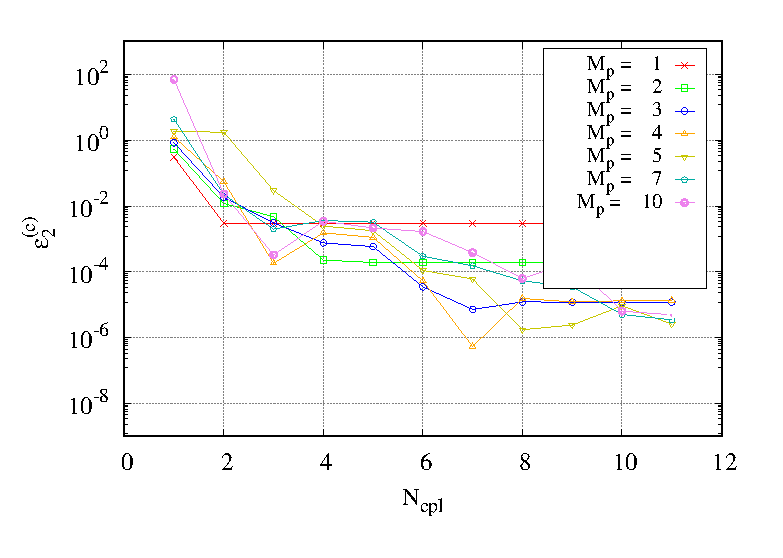
\includegraphics[width=0.485\textwidth]{figures/coupling/output_slip_err_ipu_dudz_noslip.eps}}
        \subfigure[\label{fig:err_ipu_velocity}u]
        {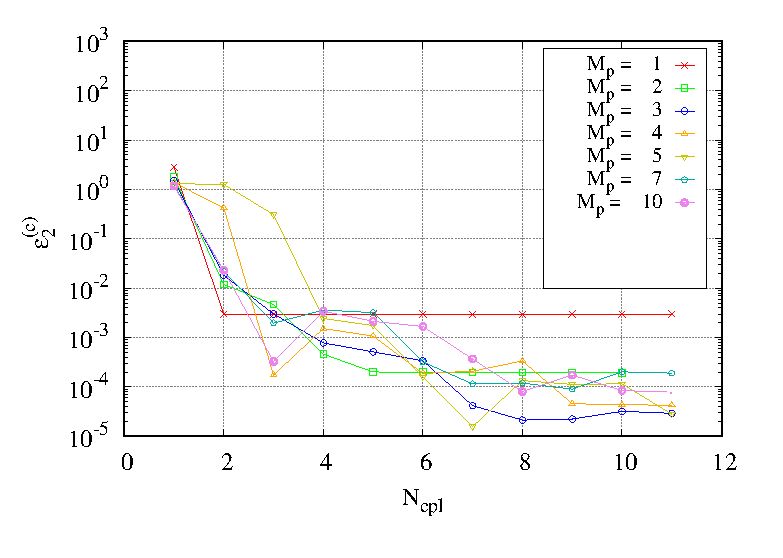
\includegraphics[width=0.485\textwidth]{figures/coupling/output_slip_err_ipu_velocity_noslip.eps}}
     \caption{erreurs dudz et velocity ipu}
    \label{fig:err_ipu_dudz_velocity}
\end{figure}
\end{frame}
%------------------------- %------------------------- 
%------------------------- %------------------------- 
% \begin{frame}{Frame Title}
%     \begin{figure}[!ht]
%      \centering
%      \subfigure[\label{fig:err_pu_dudz} dudz]
%         {\hspace{-0.2cm}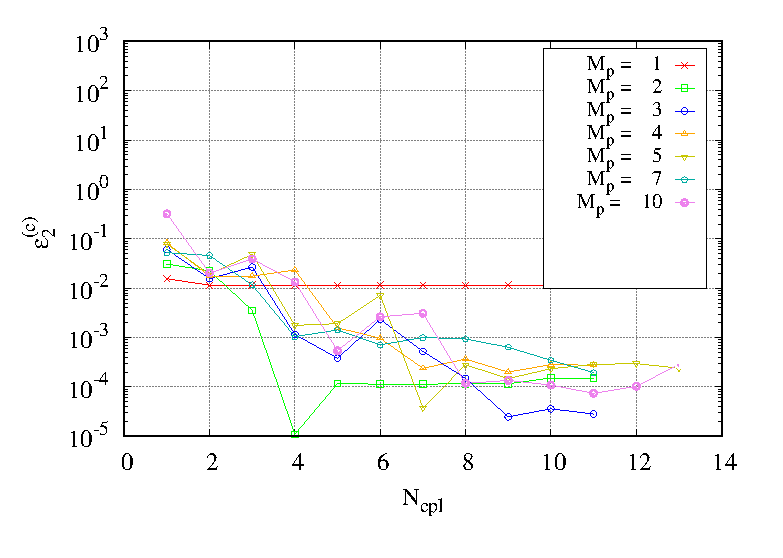
\includegraphics[width=0.49\textwidth]{figures/coupling/output_slip_err_pu_dudz.eps}}
%         \subfigure[\label{fig:err_pu_velocity}u]
%         {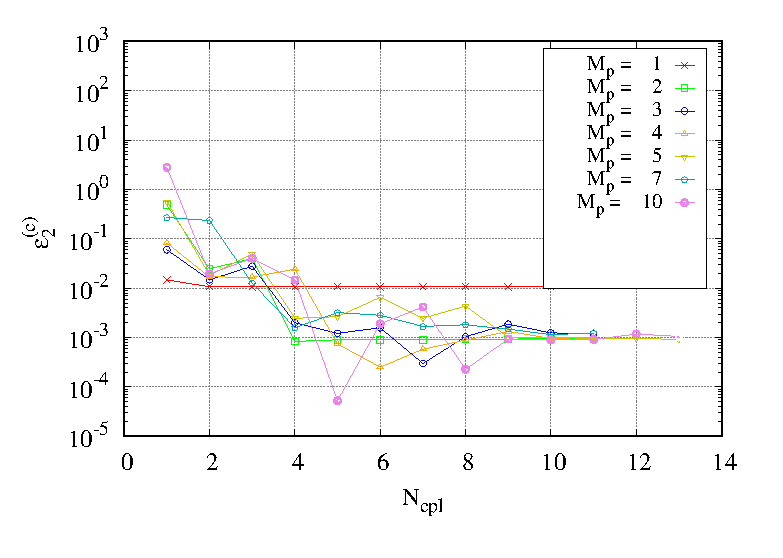
\includegraphics[width=0.49\textwidth]{figures/coupling/output_slip_err_pu_velocity.eps}}
%      \caption{erreurs dudz et velocity pu}
%     \label{fig:err_pu_dudz_velocity}
% \end{figure}
% \end{frame}

%------------------------- %------------------------- 
%------------------------- %------------------------- 
\begin{frame}{Lists -- Done list 04/11/22 }
{To do list 28/10/22  --  Done list 04/11/22}

\begin{enumerate}
    \item \textcolor{green!50!black}{R}ÉDACTION !
    \item Abstract NEGF23 à corriger
    \item \textcolor{red}{couplage 1000 : Reprise à partir d'un calcul glissement : same result}
    \item \textcolor{green!50!black}{couplage (10) : apprentissage par } $\mathcal{GP}$ : \blue{RBF,Matern32,Matren52}
    \item \textcolor{green!50!black}{maillage rectangulaire : apprentissage $f(\it{Kn},u)$}, Bayes
    \item \textcolor{green!50!black}{maillage triangulaire : apprentissage $f(\it{Kn},u)$}, Bayes
\end{enumerate}
\end{frame}
%%%%%%%%%%%%%%%%%%%%%%%%%%%%%%%%%%%%%%%%%%%%%%%%%%%%%
\begin{frame}{Couplage $f(p,u)$ : Gaussian Process : \orange{RBF, Matern32, Matren52}}
\begin{figure}[!ht]
     \centering
     % \subfigure[\label{fig:err_gp10} en 10 itérations]
     %    {\hspace{-0.2cm}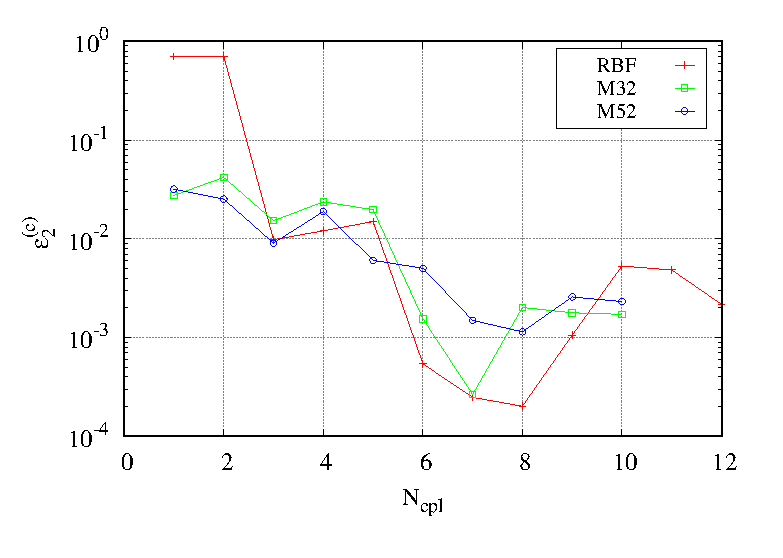
\includegraphics[width=0.49\textwidth]{figures/coupling/output_slip_err_gp_noslip.eps}}
        % \subfigure[\label{fig:err_gp20} en 20 itérations]
        {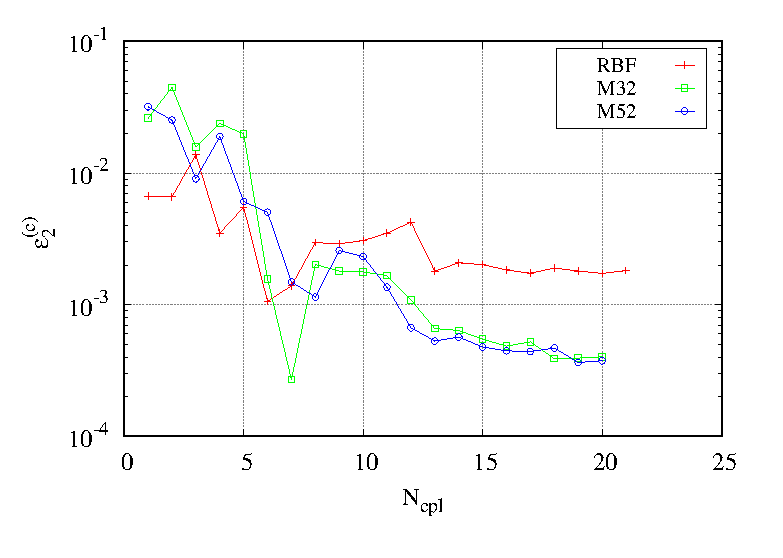
\includegraphics[width=0.65\textwidth]{figures/coupling/output_slip_err_gp_noslip_20.eps}}
     \caption{erreurs dudz sur la ligne du couplage}
    \label{fig:err_gp_case_fpu}
\end{figure}
\end{frame}
%%%%%%%%%%%%%%%%%%%%%%%%%%%%%%%%%%%%%%%%%%%%%%%%%%%%%

\begin{frame}{Couplage $f(\it Kn,u)$ : maillage rectangulaire}

\begin{table}[!ht]
    \centering
    \begin{tabular}{c|ll|cc}
    \hline
    $M_p$ & $\varepsilon_{2}^{(p)}$ & $\varepsilon_{\infty}^{(p)}$ &$\varepsilon_{2 {(u)}}^{(c)}$&$\varepsilon_{2 {(\partial_z u)}}^{(c)}$ \\
    \hline
    $1$ & $2.03\times 10^{-2}$ & $2.38\times 10^{-2}$ &  $2.99\times 10^{-3}$  & $2.99\times 10^{-3}$ \\
    $2$ & $1.28\times 10^{-3}$ & $1.62\times 10^{-2}$ &  $1.84\times 10^{-3}$  & $1.83\times 10^{-3}$ \\
    $3$ & $9.08\times 10^{-5}$ & $1.20\times 10^{-4}$ &  $1.95\times 10^{-5}$  & $1.23\times 10^{-5}$ \\
    $4$ & $5.43\times 10^{-5}$ & $1.09\times 10^{-4}$ &  $2.39\times 10^{-5}$  & $1.86\times 10^{-5}$ \\
    $5$ & $3.31\times 10^{-5}$ & $4.49\times 10^{-5}$ &  $2.89\times 10^{-5}$  & $4.56\times 10^{-6}$ \\
    $7$ & $1.53\times 10^{-4}$ & $2.28\times 10^{-4}$ &  $1.51\times 10^{-5}$  & $3.88\times 10^{-6}$ \\
    $10$ & $1.05\times 10^{-4}$ & $2.39\times 10^{-4}$ &  $6.84\times 10^{-5}$  & $8.88\times 10^{-7}$ \\
    \hline
    \end{tabular}
    \caption{Erreur de couplage $\varepsilon_{2}^{(c)}$ sur la ligne : maillage rectangulaire}
    \label{tab:ml_slip_coupling_knuh_rectangle}
\end{table}
    
\end{frame}
%%%%%%%%%%%%%%%%%%%%%%%%%%%%%%%%%%%%%%%%%%%%%%%%%%%%%
\begin{frame}{Couplage $f(\it Kn,u)$ : maillage triangulaire}

\begin{table}[!ht]
    \centering
    \begin{tabular}{c|ll|cc}
    \hline
    $M_p$ & $\varepsilon_{2}^{(p)}$ & $\varepsilon_{\infty}^{(p)}$  &$\varepsilon_{2 {(u)}}^{(c)}$&$\varepsilon_{2 {(\partial_z u)}}^{(c)}$ \\
    \hline
    $1$ & $1.45\times 10^{-1}$ & $1.30\times 10^{-1}$ &  $6.98\times 10^{-2}$  & $2.03\times 10^{-2}$ \\
    $2$ & $2.23\times 10^{-2}$ & $2.39\times 10^{-2}$ &  $1.04\times 10^{-2}$  & $3.46\times 10^{-3}$ \\
    $3$ & $4.72\times 10^{-3}$ & $5.93\times 10^{-3}$ &  $5.68\times 10^{-3}$  & $1.68\times 10^{-3}$ \\
    $4$ & $1.86\times 10^{-3}$ & $2.38\times 10^{-3}$ &  $2.92\times 10^{-3}$  & $7.26\times 10^{-4}$ \\
    % \textcolor{red}{$5$} & \textcolor{red}{$3.31\times 10^{-5}$} & \textcolor{red}{$4.49\times 10^{-5}$} &  \textcolor{red}{$2.89\times 10^{-5}$}  & \textcolor{red}{$4.56\times 10^{-6}$} \\
    $5$ &  &  &    &  \\
    $7$ & $7.71\times 10^{-4}$ & $9.51\times 10^{-4}$ &  $5.82\times 10^{-5}$  & $4.48\times 10^{-5}$ \\
    \textcolor{red}{$10$} & $7.72\times 10^{-4}$ & $9.50\times 10^{-4}$ &  $1.11\times 10^{-3}$ & $2.41\times 10^{-4}$ \\
    \hline
    \end{tabular}
    \caption{Erreur de couplage $\varepsilon_{2}^{(c)}$ sur la ligne : maillage triangulaire}
    \label{tab:ml_slip_coupling_uns_triangle}
\end{table}

\end{frame}
%%%%%%%%%%%%%%%%%%%%%%%%%%%%%%%%%%%%%%%%%%%%%%%%%%%%%
\begin{frame}{Couplage $f(\it Kn,u)$ : maillage triangulaire uniforme}

\begin{table}[!ht]
    \centering
    \begin{tabular}{c|ll|cc}
    \hline
            $M_p$ & $\varepsilon_{2}^{(p)}$ & $\varepsilon_{\infty}^{(p)}$  &$\varepsilon_{2 {(u)}}^{(c)}$&$\varepsilon_{2 {(\partial_z u)}}^{(c)}$ \\
    \hline
    $1$ & $4.37\times 10^{-2}$ & $4.74\times 10^{-2}$ &  $1.89\times 10^{-2}$  & $4.60\times 10^{-3}$ \\
    $2$ & $4.02\times 10^{-3}$ & $5.03\times 10^{-3}$ &  $3.27\times 10^{-3}$  & $4.47\times 10^{-4}$ \\
    $3$ & $4.20\times 10^{-4}$ & $4.79\times 10^{-4}$ &  $4.53\times 10^{-4}$  & $3.05\times 10^{-5}$ \\
    $4$ & $5.38\times 10^{-5}$ & $7.29\times 10^{-5}$ &  $1.27\times 10^{-4}$  & $2.51\times 10^{-5}$ \\
    \textcolor{red}{$5$} & $5.88\times 10^{-4}$ & $9.47\times 10^{-4}$ &  $5.79\times 10^{-4}$  & $1.34\times 10^{-5}$ \\
    $7$ & $6.08\times 10^{-5}$ & $1.36\times 10^{-4}$ &  $1.96\times 10^{-4}$  & $5.28\times 10^{-5}$ \\
    \textcolor{red}{$10$} & $4.97\times 10^{-4}$ & $7.18\times 10^{-4}$ &  $3.34\times 10^{-3}$ & $1.02\times 10^{-4}$ \\
    \hline
    \end{tabular}
    \caption{Erreur de couplage $\varepsilon_{2}^{(c)}$ sur la ligne : maillage triangulaire uniforme}
    \label{tab:ml_slip_coupling_unsu_triangle_uniform}
\end{table}
\end{frame}
%%%%%%%%%%%%%%%%%%%%%%%%%%%%%%%%%%%%%%%%%%%%%%%%%%%%%
%%%%%%%%%%%%%%%%%%%%%%%%%%%%%%%%%%%%%%%%%%%%%%%%%%%%%



%%%%%%%%%%%%%%%%%%%%%%%%%%%%%%%%%%%%%%%%%%%%%%%%%%%%%
\begin{frame}{Lists -- {Done list 18/11/22}}
\begin{enumerate}
    \item \textcolor{green!50!black}{RÉ}DACTION ! + Résumé NEGF23 envoyé !
    \item \textcolor{green!50!black}{maillage rectangulaire : apprentissage $f(\it{Kn},u)$}, $\mathcal{GP}$
    \item \textcolor{green!50!black}{maillage triangulaire : apprentissage $f(\it{Kn},u)$}, $\mathcal{GP}$
    \item glissement de deux cotés : 
    \item \textcolor{green!50!black}{couplage (10) : apprentissage Bayes }

\end{enumerate}
\end{frame}
%%%%%%%%%%%%%%%%%%%%%%%%%%%%%%%%%%%%%%%%%%%%%%%%%%%%%
\begin{frame}{Dev --  analytical functions (slip2)}
{Glissement de deux côtés, deux apprentissages}

\begin{equation*}
\begin{aligned}
u \left( z \right) ={\it C1}\,z+{\it C2} \quad ; \quad 
    & u \left( z \right) =u_0 + \lambda \left.\frac {\partial u}{\partial z}\right\vert_{z=0} \quad ; \quad {\it C2}&=\lambda\,{\it C1} \\ %u_0=0 \\
    & u \left( z \right) = u_p - \lambda^\prime \left.\frac {\partial u}{\partial z}\right\vert_{z=H}
    \quad ; \quad {\it C1}&={\frac {{\it u_p}}{H+\lambda^\prime+\lambda}}
\end{aligned}
\end{equation*}
\begin{equation*}
  u \left( z \right) = {\frac {{\it u_p}\, \left( \lambda+z \right) }{H+\lambda^\prime+\lambda}}
\end{equation*}

\begin{equation*}
  u \left( z^\star \right) = {\frac {{\it u_p}\, \left( {\it Kn}+z^\star \right) }{H/h_K+\it Kn^\prime+{\it Kn}}}
\end{equation*}
\end{frame}
%%%%%%%%%%%%%%%%%%%%%%%%%%%%%%%%%%%%%%%%%%%%%%%%%%%%%
%%%%%%%%%%%%%%%%%%%%%%%%%%%%%%%%%%%%%%%%%%%%%%%%%%%%%
\begin{frame}{Lists -- To do list}
{il reste}
\begin{enumerate}
    \item \textcolor{green!50!black}{RÉ}DACTION !!!!
    \item glissement de deux cotés pour $\mathcal{GP}$
    \item glissement de deux cotés avec un maillage non structuré !
    \item glissement de deux cotés avec un maillage non structuré ! pour $\mathcal{GP}$
    \item gradient de pression non nul $\nabla p \neq 0$
    \item condensation ?
    \item dynamique moléculaire ?
\end{enumerate}
\end{frame}
%%%%%%%%%%%%%%%%%%%%%%%%%%%%%%%%%%%%%%%%%%%%%%%%%%%%%
% %%%%%%%%%%%%%%%%%%%%%%%%%%%%%%%%%%%%%%%%%%%%%%%%%%%%%
% \begin{frame}{Results }
% \textbf{Results -- err}
% 	\begin{figure}
% 		\centering
% 		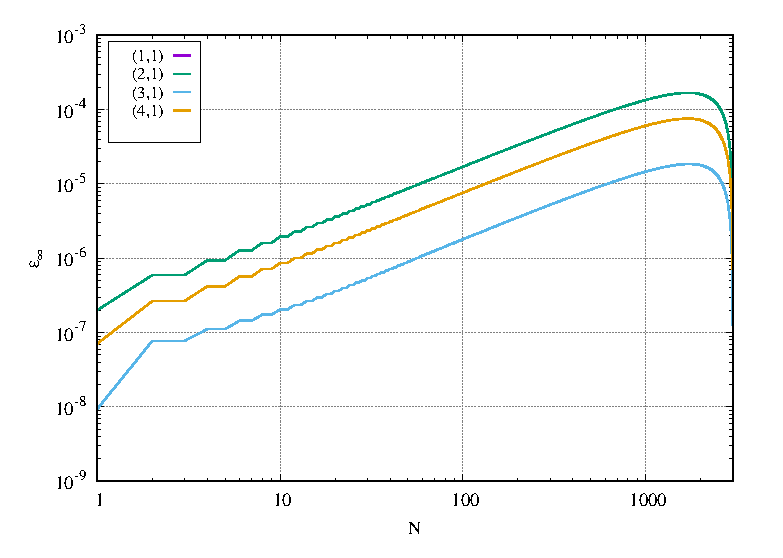
\includegraphics[,width=0.65\linewidth]{figures/err_u_nvstks.eps}
% 	\end{figure}
% \end{frame}
% %%%%%%%%%%%%%%%%%%%%%%%%%%%%%%%%%%%%%%%%%%%%%%%%%%%%%


%%%%%%%%%%%%%%%%%%%%%%%%%%%%%%%%%%%%%%%%%%%%%%%%%%%%%
% \begin{frame}{A faire}
% \begin{itemize}
% 	\item couplage avec MD
% 	\item imposer une vitesse aux molécules fluides dans lammps
% 	\item mettre le bruit ? 
% \end{itemize}
% \end{frame}




%%%%%%%%%%%%%%%%%%%%%%%%%%%%%%%%%%%%%%%%%%%%%%%%%%%%%
% \begin{frame}
% \frametitle{Basis function choice}

% \begin{equation}
% f(u_K,p)=\frac{u_K - u_P}{h+\sigma_u \lambda}\quad\mbox{où}\quad \lambda = \frac{\mu}{p}\sqrt{\frac{\pi r T}{2}}
% \end{equation}
% \begin{equation}
% 	f(u_K,p)=\frac{u_K - u_P}{h} \sum_{i=0}^{\infty} \left((-1)\sigma_u\frac{\lambda}{h}\right)^i
% \end{equation}
% \begin{minipage}{.5\textwidth}
% \hspace{-1.25cm}
% %\centering
% avec :%(données SI Dahia)
% \begin{itemize}
% 	\item $u_P$ = 0
% 	\item $\sigma_u=1$
% 	\item $h=2.05\times 10^{-7}$
% 	\item $\mu=1.78\times 10^{-5}$
% 	\item $r = 296.8$
% 	\item $T=300$
% \end{itemize}
% et bornes initiales :
% \begin{itemize}
% 	\item $p\in [ 8\times 10^{4}, 10^{5}]$
% 	\item $u_K\in [2.50, 5.07] $
% \end{itemize}%\\
% %\hspace{-1.25cm}
% \end{minipage}%
% \begin{minipage}{.5\textwidth}
% \hspace{+0.25cm}
% \centering
% \begin{minipage}[c]{0.4\linewidth} % [t] : paragraph aligned at the top
% \begin{tikzpicture}[scale=0.8]
% \draw[step=0.5cm,gray,very thin] (0,0) grid (4,4);
% \end{tikzpicture}
% \end{minipage}
% \end{minipage}
% \end{frame}


\end{document}
